\chapter{Especificación de Requisitos}

\section{Introducción}

\subsection{Propósito}

El propósito de esta especificación de requisitos es definir de manera sencilla, breve y clara las funciones y restricciones que deberá poseer el producto final que se va a desarrollar. \\

Para elaborarlo, se tendrán en cuenta las necesidades de los usuarios finales. El resultado final servirá como base para la construcción de la aplicación y se tendrá en cuenta a lo largo de todo su desarrollo. 

\subsection{Alcance}

La aplicación facilitará la toma de decisiones dentro de un grupo social, pudiendo usar opciones por defecto o personalizadas y eligiendo finalmente mediante diversos métodos de elección. A su vez, irá guardando y tomando los datos de la base de datos del sistema.

\subsection{Definiciones}

\begin{itemize}
    \item \textit{\uline{Administrador:}} Persona con acceso completo al sistema software y responsable del mantenimiento de la base de datos. De igual modo, podrá realizar las funciones de los \textit{clientes}.
    \item \textit{\uline{Cliente:}} Persona interesada en la toma de decisiones gamificada que ofrece la aplicación.
    \item \textit{\uline{Servidor:}} Equipo de cómputo en el que se implementará el sistema.
    \item \textit{\uline{Grupo:}} Conjunto de clientes que pueden tomar decisiones en común.
\end{itemize}

\section{Descripción general}

En este apartado, vamos a proporcionar una visión general del sistema. Con el objetivo, de determinar las funciones principales, datos necesarios y restricciones que afecten al desarrollo.

\subsection{Perspectiva del producto}

El sistema hará uso de una base de datos en la que se recogerá y guardará información relativa a los grupos y los distintos usuarios de la aplicación. \\

La interacción de los usuarios se llevará a cabo mediante una interfaz gráfica, la cual podrá ser accedida mediante una pantalla táctil.

\subsection{Funciones del Producto}

Las funciones principales del sistema son la F1 y F2, las cuales vamos a comentar a continuación:

\begin{itemize}
    \item Código F1: Gestión de una base de datos (permitiendo insertar, actualizar y eliminar) en la que se almacenan los miembros de cada grupo, las opciones de cada decisión por defecto y la información de los usuarios y su rol en la aplicación.
    \item Código F2: Devolver información filtrada sobre ocio a través de APIs y/o \textit{scraping}.
\end{itemize}

Asimismo, la aplicación contará con las siguientes funciones:

\begin{itemize}
    \item Creación-Edición-Eliminación: Se usará tanto para usuarios como para grupos y opciones de las decisiones. 
    \item Añadir-Eliminar: Podrá utilizarse sobre los miembros de un grupo.
    \item Historial: Se podrán ver las votaciones anteriores, con la posibilidad de repetirlas.
\end{itemize}


\subsection{Características de los usuarios}

Es recomendable que los usuarios tengan conocimientos básicos de informática y estén familiarizados con el uso de aplicaciones en dispositivos móviles.

\subsection{Restricciones}

Las principales restricciones que debe cumplir el sistema son RES1, RES3 y RES6, las cuales vamos a comentar a continuación:

\begin{itemize}
    
    \item Código RES3: Siempre debe haber al menos un administrador creado en el sistema.
    \item Código RES4: Un administrador no podra cambiar su propio rol o eliminarse.
\end{itemize}

\begin{comment}
\begin{itemize}
    \item Código RES1: Una vez insertado un usuario con un email específico en la base de datos, no se podrá registrar un usuario con el mismo  email (debido a la duplicidad).
    \item Código RES2: Una vez añadido un usuario en un grupo, no se podrá volver a insertar(a causa de que ya pertenece a él).
    \item Código RES3: Siempre debe haber al menos un administrador creado en el sistema.
    \item Código RES4: Un administrador no podra cambiar su propio rol o eliminarse.
    \item Código RES5: El email introducido deberá contar con un formato específico.
    \item Código RES6: El nombre de usuario no podrá estar repetido en el sistema.
    \item Código RES7: Para que exista un grupo, debe haber en él al menos un miembro.
    \item Código RES8: No se permitirá almacenar información personal en texto plano.
    \item Código RES9: Un usuario solo podrá registrar su voto una vez por votación
\end{itemize}
\end{comment}

\subsection{Suposiciones y dependencias}

Se asume que el sistema operativo de destino es Android o iOS y que estará disponible y correctamente configurado en los equipos donde se instalará la aplicación.

\section{Requerimientos específicos}

\subsection{Requisitos funcionales}

\begin{itemize}
    \item Código REQ1: Registro de decisión $\rightarrow$ El administrador podrá registrar decisiones por defecto y guardarlas en la base de datos. Para ello, tendrá como mínimo que rellenar el ID de la decisión, el título y la lista de opciones.
    \item Código REQ2: Creación de opciones $\rightarrow$ El sistema permitirá que los usuarios añadan opciones a las decisiones, contando cada una con título y opcionalmente descripción e imagen.
    \item Código REQ3: Subida de imágenes $\rightarrow$ Los usuarios podrán adjuntar imágenes en el sistema.
    \item Código REQ4: Mecanismo de votación $\rightarrow$ El sistema permitirá al creador de la votación elegir el tipo de votación, pudiendo elegir entre una lista de opciones como ranking, consenso, pesos, etc.
    \item Código REQ5: Límite de tiempo $\rightarrow$ El creador de la votación podrá fijar un tiempo máximo para que el resto de miembros ejerza su derecho al voto.
    \item Código REQ6: Filtrado $\rightarrow$ El sistema contará con sistemas de filtrado y búsqueda mediante APIs o scraping para aportar opciones en la votación.
    \item Código REQ7: Perfil del usuario $\rightarrow$ El usuario dispondrá de una cuenta personal asociada a él que podrá crear, modificar y eliminar.
    \item Código REQ8: Login $\rightarrow$ Todos los usuarios entrarán al sistema mediante un inicio de sesión compuesto por nombre de usuario y contraseña.
    \item Código REQ9: Administración $\rightarrow$ El administrador dispondrá de acceso total a los datos guardados en el sistema pudiendo modificarlos a voluntad. 
\end{itemize}

\subsection{Requisitos no funcionales}

\begin{itemize}
    \item d
\end{itemize}


\subsection{Requisitos de interfaces externas}

\begin{itemize}
    \item Código REQ6: Interfaces de usuario $\rightarrow$ Se podrá comunicar con el usuario para aprovechar los requisitos del sistema, el usuario indicará al sistema las operaciones que desea realizar e introducirá los datos que el sistema le pida.
    \item Código REQ7: Interfaces del software $\rightarrow$ La comunicación entre los módulos del sistema se realizará mediante bases de datos.
    \item Código REQ8: Mantenibilidad $\rightarrow$ El sistema será diseñado para que tenga fácil mantenimiento, con el objetivo de que pueda ser ampliado y corregido si es necesario.
\end{itemize}

\subsection{Interfaces externas}

\begin{itemize}
    \item Interfaz de usuario: Será de facil manejo, contando con una interfaz intuitiva. Tendrá una apariencia similar a los bocetos mostrados en las Figuras \ref{fig:boceto_homepage} y \ref{fig:boceto_grupopage}.

    \begin{figure}[ht]
        \centering
        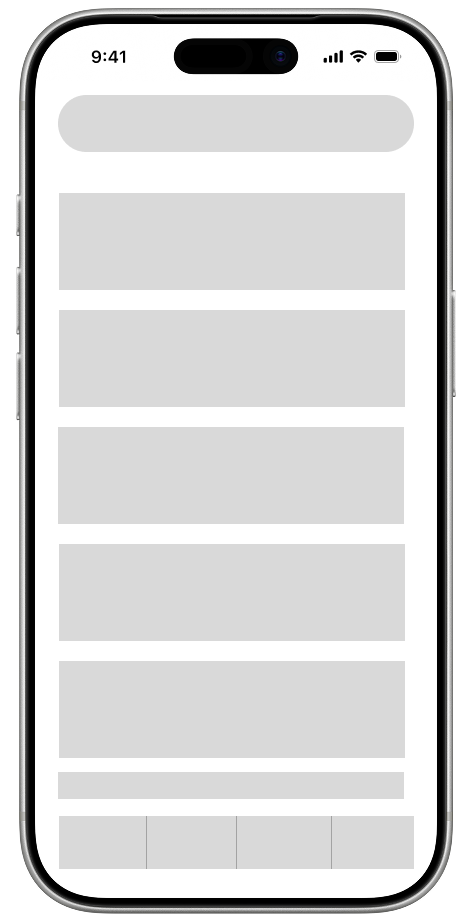
\includegraphics[width=\tamApps\textwidth]{figuras/bocetos/homepage.png}
        \caption{Boceto de la página principal}
        \label{fig:boceto_homepage}
    \end{figure}

    \begin{figure}[ht]
        \centering
        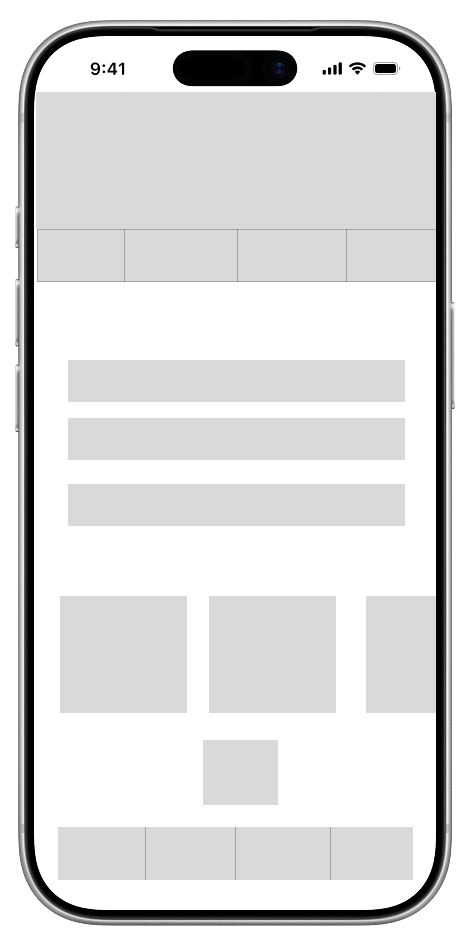
\includegraphics[width=\tamApps\textwidth]{figuras/bocetos/grupopage.png}
        \caption{Boceto de la página principal de un grupo}
        \label{fig:boceto_grupopage}
    \end{figure}
    
    \item Interfaz hardware: Será desarrollado para poder usarse con una pantalla táctil. Asimismo, no hará falta una interfaz hardware específica para ejecutarlo.
    \item Interfaz software: La interfaz software utilizada será la proporcionada por los Sistemas Operativos que vamos a utilizar, en este caso Android e iOS. 
    \item Comunicación entre interfaces: La comunicación con funciones del sistema se realizará mediante \textit{Platform Channels}, ya sea a través de \textit{plugins} de la comunidad o mediante implementaciones personalizadas.
\end{itemize}
